\documentclass[11pt]{article}
\usepackage{amsfonts}
\usepackage{amsmath}
\usepackage{latexsym}
\usepackage{hyperref}
\usepackage{pdfpages}
\usepackage{tikz}
\usepackage{wrapfig}
\usepackage{fancyvrb}
\usepackage{fontspec}
\usepackage{fancybox}
\usepackage{listings}
\usepackage{enumitem}
\usepackage{ducksay}
\usepackage{xcolor}
\usepackage{amssymb}
\usepackage{graphicx}
\usepackage{parskip}
\usepackage{tabularray}
\usepackage{subcaption}
\usepackage{tikz-qtree}
\usetikzlibrary{automata,arrows}
\graphicspath{ {./images/} }
\setlength{\oddsidemargin}{.25in}
\setlength{\evensidemargin}{.25in}
\setlength{\textwidth}{6in}
\setlength{\topmargin}{-0.4in}
\setlength{\textheight}{8.5in}
\setlength{\parindent}{0cm}
\UseTblrLibrary{booktabs}

\def\squarebox#1{\hbox to #1{\hfill\vbox to #1{\vfill}}}
\def\qed{\hspace*{\fill}
  \vbox{\hrule\hbox{\vrule\squarebox{.667em}\vrule}\hrule}}
\newenvironment{solution}{\begin{trivlist}\item[]{\bf Solution:}}
  {\qed \end{trivlist}}
\newenvironment{solsketch}{\begin{trivlist}\item[]{\bf Solution Sketch:}}
  {\qed \end{trivlist}}
\newenvironment{proof}{\begin{trivlist}\item[]{\bf Proof:}}
  {\qed \end{trivlist}}

\newtheorem{theorem}{Theorem}
\newtheorem{corollary}[theorem]{Corollary}
\newtheorem{lemma}[theorem]{Lemma}
\newtheorem{observation}[theorem]{Observation}
\newtheorem{remark}[theorem]{Remark}
\newtheorem{proposition}[theorem]{Proposition}
\newtheorem{definition}[theorem]{Definition}
\newtheorem{Assertion}[theorem]{Assertion}
\newtheorem{fact}[theorem]{Fact}
\newtheorem{hypothesis}[theorem]{Hypothesis}
% \newtheorem{observation}[theorem]{Observation}
% \newtheorem{proposition}[theorem]{Proposition}
\newtheorem{claim}[theorem]{Claim}
\newtheorem{assumption}[theorem]{Assumption}

% Put more macros here, as needed.
\newcommand{\al}{\alpha}
\newcommand{\Z}{\mathbb Z}
\newcommand{\jac}[2]{\left(\frac{#1}{#2}\right)}
\newcommand{\set}[1]{\#1}
\newcommand{\evenSpace}{\vspace*{\stretch{1}}}
% Assignment header with the appropriate information
% 1st arg: Group member names
% 2nd arg: Assignment #
\newcommand{\header}[2]{
  \begin{center}
    \setlength\fboxsep{.3cm}
    \doublebox{
      \parbox{\dimexpr\linewidth-2\fboxsep-2\fboxrule} {
        #1 \\
        COSC 336 \\
        \today \par
        \centering{\huge{Assignment #2}}
      }}
  \end{center}
}

\def\ppt{{\sf PPT}}
\def\poly{{\sf poly}}
\def\negl{{\sf negl}}
\def\owf{{\sf OWF}}
\def\owp{{\sf OWP}}
\def\tdp{{\sf TDP}}
\def\prg{{\sf PRG}}
\def\prf{{\sf PRF}}
\definecolor{variableColor}{HTML}{AA7700}
\definecolor{commentsColor}{rgb}{0.497495, 0.497587, 0.497464}
\definecolor{keywordsColor}{rgb}{0.00000, 0.000000, 1.500000}
\definecolor{stringColor}{rgb}{0.558215, 0.000000, 0.135316}
\lstset {
  backgroundcolor=\color{white},   % choose the background color; you must add \usepackage{color} or \usepackage{xcolor}
  basicstyle=\ttfamily,        % the size of the fonts that are used for the code
  breakatwhitespace=false,         % sets if automatic breaks should only happen at whitespace
  breaklines=true,                 % sets automatic line breaking
  captionpos=b,                    % sets the caption-position to bottom
  commentstyle=\color{commentsColor}\textit,    % comment style
  extendedchars=true,              % lets you use non-ASCII characters; for 8-bits encodings only, does not work with UTF-8
  frame=tblr, % adds a frame around the code
  % framexleftmargin=1.5em,
  keepspaces=true,                 % keeps spaces in text, useful for keeping indentation of code (possibly needs columns=flexible)
  keywordstyle=\color{keywordsColor}\bfseries,       % keyword style
  language=Java,                   % the language of the code (can be overrided per snippet)
  otherkeywords={*,...},           % if you want to add more keywords to the set
  numbers=none,                    % where to put the line-numbers; possible values are (none, left, right)
  numbersep=5pt,                   % how far the line-numbers are from the code
  numberstyle=\tiny\color{commentsColor}, % the style that is used for the line-numbers
  rulecolor=\color{black},         % if not set, the frame-color may be changed on line-breaks within not-black text (e.g. comments (green here))
  showspaces=false,                % show spaces everywhere adding particular underscores; it overrides 'showstringspaces'
  showstringspaces=false,          % underline spaces within strings only
  showtabs=false,                  % show tabs within strings adding particular underscores
  stepnumber=1,                    % the step between two line-numbers. If it's 1, each line will be numbered
  stringstyle=\color{stringColor}, % string literal style
  tabsize=2,                   % sets default tabsize to 2 spaces
  % title=Solution to the Longest increasing subsequence problem,
  % show the filename of files included with \lstinputlisting; also try caption instead of title
  columns=fixed                    % Using fixed column width (for e.g. nice alignment)
}
\begin{document}
\header{Luis Gascon, Ethan Webb, Femi Dosumu}{8}
\textbf{Exercise 1.}

Describe in plain English (a short paragraph with at most 5-6 lines should be enough) an  algorithm for the following task:
\medskip

\emph{Input}: A directed graph $G = (V,E)$, and a node $u \in V$.

\emph{Goal:}  Output 1 if there is a path from  every  $v \in G$ to $u$ (so if $u$ is reachable from any other node), and output $0$ otherwise.
\medskip

Your algorithm should have runtime $O(n+m)$.  (Hint: Use an idea that we have seen for similar connectivity problems in directed graphs.)

\newpage

\textbf{Exercise 2.}

We have seen that Dijkstra's algorithm can be implemented in two ways: Variant (a) uses an array to store the $dist[]$ values of the unknown nodes, and Variant (b) uses a MIN-HEAP to store these values.
\medskip

(a) Suppose in your application $m \le 3n$. Which variant gives a faster runtime?  Justify your answer.


(b) Suppose in your application $m \ge n^2/3$. Which variant gives a faster runtime?  Justify your answer.
\newpage

Our algorithm starts off by initializing two integer arrays \verb|dist| and \verb|npath|.

\begin{lstlisting}
int[] dist = new int[g.n];
int[] npath = new int[g.n];

for (int i = 0; i < g.n; i++) {
    dist[i] = Integer.MAX_VALUE;
    npath[i] = 0;
}
\end{lstlisting}

I've set the undiscovered nodes to have a distance of infinity, and in this case, the maximum integer value that Java supports.

\newpage
The algorithm in its entirety.
\begin{lstlisting}
static void getShortestPath(Adj_List_Graph g, int s) {
  int[] dist = new int[g.n];
  int[] npath = new int[g.n];

  for (int i = 0; i < g.n; i++) {
      dist[i] = Integer.MAX_VALUE;
      npath[i] = 0;
  }

  Queue<Integer> queue = new LinkedList<Integer>();

  dist[s] = 0;
  npath[s] = 1;
  queue.add(s);
  while (!queue.isEmpty()) {
      int p = queue.poll();
      List<Integer> neighbors = g.adj.get(p);
      for (int v : neighbors) {
          if (dist[v] == Integer.MAX_VALUE) {
              dist[v] = dist[p] + 1;
              npath[v] = npath[p];
              queue.add(v);
          }

          else if (dist[v] == dist[p] + 1)
              npath[v] += npath[p];

      }
  }

  for (int index = 1; index < g.n; index++)
      System.out.printf("dist[%d] = %d \t npath[%d] = %d%n",
              index, dist[index], index, npath[index]);

}
\end{lstlisting}

Program output can be found on the next page.
\newpage
\begin{lstlisting}
G1 results:

dist[1] = 0 	 npath[1] = 1
dist[2] = 1 	 npath[2] = 1
dist[3] = 1 	 npath[3] = 1
dist[4] = 1 	 npath[4] = 1
dist[5] = 2 	 npath[5] = 2
dist[6] = 2 	 npath[6] = 1
dist[7] = 3 	 npath[7] = 3

G2 results:

dist[1] = 0 	 npath[1] = 1
dist[2] = 1 	 npath[2] = 1
dist[3] = 1 	 npath[3] = 1
dist[4] = 1 	 npath[4] = 1
dist[5] = 1 	 npath[5] = 1
dist[6] = 1 	 npath[6] = 1
dist[7] = 2 	 npath[7] = 5
dist[8] = 3 	 npath[8] = 5
dist[9] = 3 	 npath[9] = 5
\end{lstlisting}
To visually reflect one of our solutions, namely dist[7] and npath[7] of \verb|G2|, we'll highlight the paths.
\begin{center}
  \begin{tikzpicture}[>=stealth',shorten >=1pt,auto,node distance=2.0cm,scale=0.3]][h]
    %\begin{tikzpicture}[shorten >=1pt,auto,node distance=2.8cm]][h]
    \node[state] (1) {$1$};
    \node[state] (2) [below left of =1] {$2$};
    \node[state] (3) [right of=2] {$3$};
    \node[state] (4) [right of=3] {$4$};
    \node[state] (5) [right of=4] {$5$};
    \node[state] (6) [right  of=5] {$6$};
    \node[state] (7) [below of=4] {$7$};
    \node[state] (8) [below of=7] {$8$};
    \node[state] (9) [right of =8] {$9$};

    \path[-]
    (1) edge (2)
    (1) edge (3)
    (1) edge (4)
    (1) edge (5)
    (1) edge (6)
    (7) edge (2)
    (7) edge (3)
    (7) edge (4)
    (7) edge (5)
    (7) edge (6)
    (7) edge (8)
    (7) edge (9)
    ;

  \end{tikzpicture}
\end{center}
\end{document}
